% В этом документе преамбула

%%% Работа с русским языком
\usepackage{cmap}					% поиск в PDF
\usepackage{mathtext} 				% русские буквы в формулах
\usepackage[T2A]{fontenc}			% кодировка
\usepackage[utf8]{inputenc}			% кодировка исходного текста
\usepackage[english,russian]{babel}	% локализация и переносы
\usepackage{indentfirst}			% чтобы первый абзац в разделе отбивался красной строкой
\frenchspacing						% тонкая настройка пробелов

%%% Приведение начертания букв и знаков к русской типографской традиции
\renewcommand{\epsilon}{\ensuremath{\varepsilon}}
\renewcommand{\phi}{\ensuremath{\varphi}}			% буквы "эпсилон"
\renewcommand{\kappa}{\ensuremath{\varkappa}}		% буквы "каппа"
\renewcommand{\le}{\ensuremath{\leqslant}}			% знак меньше или равно
\renewcommand{\leq}{\ensuremath{\leqslant}}			% знак меньше или равно
\renewcommand{\ge}{\ensuremath{\geqslant}}			% знак больше или равно
\renewcommand{\geq}{\ensuremath{\geqslant}}			% знак больше или равно
\renewcommand{\emptyset}{\varnothing}				% знак пустого множества

%%% Дополнительная работа с математикой
\usepackage{amsmath,amsfonts,amssymb,amsthm,mathtools} % AMS
\usepackage{icomma} % "Умная" запятая: $0,2$ --- число, $0, 2$ --- перечисление

%% Номера формул
\mathtoolsset{showonlyrefs=true} % Показывать номера только у тех формул, на которые есть \eqref{} в тексте.

%% Свои команды

% операции, не определённые (или имеющие иные обохначения) в мат. пакетах
\DeclareMathOperator{\sgn}{\mathop{sgn}}				% ф-ия sgn
\renewcommand{\tg}{\mathop{\mathrm{tg}}\nolimits}		% обозначение тангенса

%% Перенос знаков в формулах (по Львовскому)
\newcommand*{\hm}[1]{#1\nobreak\discretionary{}
{\hbox{$\mathsurround=0pt #1$}}{}}

%%% Работа с картинками
\usepackage{graphicx}  % Для вставки рисунков
\graphicspath{{images/}{images2/}}  % папки с картинками
\setlength\fboxsep{3pt} % Отступ рамки \fbox{} от рисунка
\setlength\fboxrule{1pt} % Толщина линий рамки \fbox{}
\usepackage{wrapfig} % Обтекание рисунков текстом

%%% Работа с таблицами
\usepackage{array,tabularx,tabulary,booktabs} % Дополнительная работа с таблицами
\usepackage{longtable}  % Длинные таблицы
\usepackage{multirow} % Слияние строк в таблице

%%% Теоремы
\theoremstyle{plain} % Это стиль по умолчанию, его можно не переопределять.
\newtheorem{theorem}{Теорема}[section]
\newtheorem{lemma}{Лемма}[section]
\newtheorem{definition}[theorem]{Определение}
\newtheorem{property}{Свойство}
 
\theoremstyle{definition} % "Определение"
\newtheorem{corollary}{Следствие}[theorem]
\newtheorem{exmp}{Пример}[section]
 
\theoremstyle{remark} % "Примечание"
\newtheorem*{nonum}{Решение}
\newtheorem*{evidence}{Доказательство}
\newtheorem*{remark}{Примечание}

%%% Программирование
\usepackage{etoolbox} % логические операторы

%%% Страница
\usepackage{extsizes} % Возможность сделать 14-й шрифт
\usepackage{geometry} % Простой способ задавать поля
	\geometry{top=25mm}
	\geometry{bottom=35mm}
	\geometry{left=35mm}
	\geometry{right=20mm}

%\usepackage{fancyhdr} % Колонтитулы
% 	\pagestyle{fancy}
 	%\renewcommand{\headrulewidth}{0pt}  % Толщина линейки, отчеркивающей верхний колонтитул
% 	\lfoot{Нижний левый}
% 	\rfoot{Нижний правый}
% 	\rhead{Верхний правый}
% 	\chead{Верхний в центре}
% 	\lhead{Верхний левый}
%	\cfoot{Нижний в центре} % По умолчанию здесь номер страницы

\usepackage{setspace} % Интерлиньяж (межстрочные интервалы)
%\onehalfspacing % Интерлиньяж 1.5
%\doublespacing % Интерлиньяж 2
%\singlespacing % Интерлиньяж 1

\usepackage{lastpage} % Узнать, сколько всего страниц в документе.

\usepackage{soulutf8} % Модификаторы начертания

\usepackage{hyperref}
\usepackage[usenames,dvipsnames,svgnames,table,rgb]{xcolor}
\hypersetup{				% Гиперссылки
    unicode=true,           % русские буквы в раздела PDF
    pdftitle={Заголовок},   % Заголовок
    pdfauthor={Автор},      % Автор
    pdfsubject={Тема},      % Тема
    pdfcreator={Создатель}, % Создатель
    pdfproducer={Производитель}, % Производитель
    pdfkeywords={keyword1} {key2} {key3}, % Ключевые слова
    colorlinks=true,       	% false: ссылки в рамках; true: цветные ссылки
    linkcolor=MidnightBlue,          % внутренние ссылки
    citecolor=black,        % на библиографию
    filecolor=magenta,      % на файлы
    urlcolor=blue           % на URL
}

\usepackage{csquotes} % Еще инструменты для ссылок

%\usepackage[style=authoryear,maxcitenames=2,backend=biber,sorting=nty]{biblatex}

\usepackage{multicol} % Несколько колонок

%%% Работа с графикой
\usepackage{tikz}
\usetikzlibrary{calc}
\usepackage{tkz-euclide}
\usetikzlibrary{arrows}
\usepackage{pgfplots}
\usepackage{pgfplotstable}

%%% Настройка подписей к плавающим объектам
\usepackage{floatrow}	% размещение
\usepackage{caption}	% начертание
\captionsetup[figure]{labelfont=bf,textfont=it,font=footnotesize}	% нумерация и надпись курсивом
% для подфигур: заголовок подписи полужирный, текст заголовка обычный
% выравнивание является неровным (т.е. выровненным по левому краю)
% singlelinecheck = off означает, что настройка выравнивания используется, даже если заголовок имеет длину только одну строку.
% если singlelinecheck = on, то заголовок всегда центрируется, когда заголовок состоит только из одной строки.
\captionsetup[subfigure]{labelfont=bf,textfont=normalfont,singlelinecheck=off,justification=raggedright}

%%% Stuff для графиков и рисунков



\title{Теория вероятностей и мат. статистика}
\date{25.04.2020}
\author{Почаев Никита Алексеевич, гр. 8381 \\ \href{mailto:pochaev.nik@gmail.com}{pochaev.nik@gmail.com} \\ Преподаватель: Малов Сергей Васильевич}

\begin{document}
	
\renewcommand{\figurename}{Рисунок}

\maketitle

\section*{Случайные вектора}

$\vec{\xi}: (\Omega, \mathcal{F}) \to (\mathbb{R}^n, \mathfrak{D}_n)$ (или $\xi: \Omega \to \mathbb{R}^n$ - измеримая функция).

$\vec{\xi} = (\xi_1, \dots, \xi_n)$, $\xi_i$ - компоненты случайного вектора $\vec{\xi}$.

$\mathcal{P}_{\xi}: \mathfrak{D}_n \to \mathfrak{D}_n$, так что $\mathcal{P}_{\xi}(I_1 \times \dots \times I_n) = P(\omega: \vec{\xi}(\omega) \in I_1 \times \dots \times I_n) = P(\xi_1 \in I_1, \dots, \xi_n \in I_n)$ - распределение вектора $\vec{\xi}$.

$F_{\xi}: \mathbb{R}^n \to [0,1]$, так что $F_{\xi}(x_1, \dots, x_n) = P(\xi_1 < x_1, \dots, \xi_n < x_n)$ - функция распределения.

$\vec{\xi}$ - дискретный (имеет дискретное распределение), если $\exists \{ \vec{a_j} \}_{j \in T}$ - не более, чем счетное множество, такое что
\[ P(\vec{\xi} \in \{ \vec{a_j} \}_{j \in T}) = \sum_{j \in T} P(\vec{\xi} = \vec{a_j}) = 1, a_j = (a_{1j}, \dots, a_{nj}) \in \mathbb{R}^n \]

$\vec{\xi}$ - абсолютно непрерывный, если $\exists p_{\xi}(\vec{x}) \ge 0$ (плотность распределения)
\[ F_{\xi} (x_1 \dots x_n) = \int_{- \infty}^{x_1} \dots \int_{- \infty}^{x_n} p_{\xi} (\vec{x}) d \vec{x} \]

\section*{Задача 2.}

\noindent\textit{\textbf{Условие:}}

\begin{table}[H]
	\centering
	\begin{tabular}{|c|c|c|c|}
		\hline
		\diagbox{Знач.  $\xi_1$}{Знач. $\xi_2$} 				  & -1   & 0    & 1   \\ \hline
		-1                                                        & 0.05 & 0.1  & 0.1 \\ \hline
		0                                                         & 0.1  & 0.05 & 0.2 \\ \hline
		1                                                         & 0.1  & 0.1  & 0.2 \\ \hline
	\end{tabular}
\end{table}

Найти:
\begin{enumerate}
	\item[а)] Функцию распределения $\xi_1$;
	\item[б)] Функцию распределения $\xi_2$;
	\item[в)] Функцию распределения $\xi_1-\xi_2$;
	\item[г)] Распределение $\xi_1^2 + \xi_2^2$;
	\item[д)] Распределение $(\xi_1^2, \xi_1-\xi_2^2)$.
\end{enumerate}

\noindent\textit{\textbf{Решение:}}

\begin{enumerate}
	\item[а)]
	Таблица распределения $\xi_1$ имеет следующий вид (суммы по строкам):
	\begin{table}[H]
		\centering
		\begin{tabular}{|c|c|c|c|}
			\hline
			$k$            & -1                & 0                 & 1               \\ \hline
			$P(\xi_1 = k)$ & 0.05+0.1+0.1=0.25 & 0.1+0.05+0.2=0.35 & 0.1+0.1+0.2=0.4 \\ \hline
		\end{tabular}
	\end{table}
	Таким образом, функция распределения:
	\[
	F_{\xi_1}(x) =
	\begin{cases}
		0, &x \le -1 \\
		\textcolor{gray}{0+0.25=}0.25, &x \in (-1, 0] \\
		\textcolor{gray}{0.25+0.35=}0.6, &x \in (0, 1] \\
		\textcolor{gray}{0.6+0.4=}1, &x > 1
	\end{cases}
	\]
	\item[б)]
	Таблица распределения $\xi_2$ имеет следующий вид (суммы по столбцам):
	\begin{table}[H]
		\centering
		\begin{tabular}{|c|c|c|c|}
			\hline
			$k$            & -1                & 0                 & 1               \\ \hline
			$P(\xi_2 = k)$ & 0.05+0.1+0.1=0.25 & 0.1+0.05+0.1=0.25 & 0.1+0.2+0.2=0.5 \\ \hline
		\end{tabular}
	\end{table}
	Таким образом, функция распределения:
	\[
	F_{\xi_2}(x) =
	\begin{cases}
		0, &x \le -1 \\
		\textcolor{gray}{0+0.25=}0.25, &x \in (-1, 0] \\
		\textcolor{gray}{0.25+0.25=}0.5, &x \in (0, 1] \\
		\textcolor{gray}{0.5+0.5=}1, &x > 1
	\end{cases}
	\]
	\item[в)]
	Носитель распределения случайной величины:
	\[ \supp (\xi_1) = \{ -1, 0, 1 \}, \supp (\xi_2) = \{ -1, 0, 1 \} \Rightarrow \supp(\xi_1 - \xi_2) = \{ -2, -1, 0, 1, 2 \} \]
	Найдём таблицу распределения:
	\[ P(\xi_1 - \xi_2 = -2) = P(\xi_1 = -1, \xi_2 = 1) = 0.1 \]
	\[ P(\xi_1 - \xi_2 = -1) = P(\xi_1 = -1, \xi_2 = 0) + P(\xi_1 = 0, \xi_2 = 1) = 0.1 + 0.2 = 0.3 \]
	\[ P(\xi_1 - \xi_2 = 0) = P(\xi_1 = -1, \xi_2 = -1) + P(\xi_1 = 1, \xi_2 = 1) + P(\xi_1 = 0, \xi_2 = 0) = 0.05 + 0.05 + 0.2 = 0.3 \]
	\[ P(\xi_1 - \xi_2 = 1) = P(\xi_1 = 1, \xi_2 = 0) + P(\xi_1 = 0, \xi_2 = -1) = 0.1 + 0.1 = 0.2 \]
	\[ P(\xi_1 - \xi_2 = 2) = P(\xi_1 = 1, \xi_2 = -1) = 0.1 \]
	Итак
	\begin{table}[H]
		\centering
		\begin{tabular}{|c|c|c|c|c|c|}
			\hline
			$k$                	   & -2  & -1  & 0   & 1   & 2   \\ \hline
			$P(\xi_1 - \xi_2) = k$ & 0.1 & 0.3 & 0.3 & 0.2 & 0.1 \\ \hline
		\end{tabular}
	\end{table}
	Функция распределения:
	\[
	F_{\xi_1 - \xi_2}(x) =
	\begin{cases}
		0, & x \le -2 \\
		\textcolor{gray}{0+0.1=}0.1, &x \in (-2, -1] \\
		\textcolor{gray}{0.1+0.3=}0.4, &x \in (-1, 0] \\
		\textcolor{gray}{0.4+0.3=}0.7, &x \in (0, 1] \\
		\textcolor{gray}{0.7+0.2=}0.9, &x \in (1, 2] \\
		\textcolor{gray}{0.9+0.1=}1, &x > 2
	\end{cases}
	\]
	\item[г)]
	Носитель распределения случайной величины:
	\[ \supp(\xi_1) = \{ -1, 0, 1 \}, \supp(\xi_2) = \{ -1, 0, 1 \} \Rightarrow \supp(\xi_1^2 + \xi_2^2) = \{ 0, 1, 2 \} \]
	Найдём таблицу распределения:
	\[ P(\xi_1^2 + \xi_2^2 = 0) = P(\xi_1 = 0, \xi_2 = 0) = 0.05 \]
	\[ P(\xi_1^2 + \xi_2^2 = 1) = P(\xi_1 = 1, \xi_2 = 0) + P(\xi_1 = 0, \xi_2 = 1) + P(\xi_1 = -1, \xi_2 = 0) + P(\xi_1 = 0, \xi_2 = -1) = \]
	\[= 0.1 + 0.2 + 0.1 + 0.1 = 0.5 \]
	\[ P(\xi_1^2 + \xi_2^2 = 2) = P(\xi_1 = 1, \xi_2 = 1) + P(\xi_1 = -1, \xi_2 = -1) + P(\xi_1 = -1, \xi_2 = 1) + P(\xi_1 = 1, \xi_2 = -1) = \]
	\[= 0.05 + 0.2 + 0.1 + 0.1 = 0.45 \]
	Итак
	\begin{table}[H]
		\centering
		\begin{tabular}{|c|c|c|c|}
			\hline
			$k$                        & 0    & 1   & 2    \\ \hline
			$P(\xi_1^2 + \xi_2^2) = k$ & 0.05 & 0.5 & 0.45 \\ \hline
		\end{tabular}
	\end{table}
	Функция распределения:
	\[
	F_{\xi_1^2 + \xi_2^2} =
	\begin{cases}
		0, &x \le 0 \\
		\textcolor{gray}{0+0.05=}0.05, &x \in (0, 1] \\
		\textcolor{gray}{0.05+0.5=}0.55, &x \in (1, 2] \\
		\textcolor{gray}{0.55+0.45=}1, &x > 2
	\end{cases}
	\]
	\item[д)]
	Носитель распределения случайной величины:
	\[ \supp (\xi_1) = \{ -1, 0, 1 \}, \supp (\xi_2) = \{ -1, 0, 1 \} \Rightarrow \supp (\xi_1 - \xi_2^2) = \{ -2, -1, 0, 1 \} \]
	Таблица распределения:
	\[\xi_2 \in \{ -1, 1 \} \Rightarrow P(\xi_1^2 + \xi_2^2 = -2) = 0.15 \]
	\[ \xi_2 = 0 \Rightarrow P(\xi_1^2 + \xi_2^2 = -1) = 0.1 \]
	\[ \xi_2 \in \{ -1, 1 \} \Rightarrow P(\xi_1^2 + \xi_2^2 = -1) = 0.3 \]
	\[ \xi_2 = 0 \Rightarrow P(\xi_1^2 + \xi_2^2 = 0) = 0.05 \]
	\[ \xi_2 \in \{ -1, 1 \} \Rightarrow P(\xi_1^2 + \xi_2^2 = 0) = 0.3 \]
	\[ \xi_2 = 0 \Rightarrow P(\xi_1^2 + \xi_2^2 = 1) = 0.1 \]
	\begin{table}[H]
		\centering
		\begin{tabular}{|c|c|c|c|c|}
			\hline
			\diagbox{Знач. $\xi_1$}{Знач. $\xi-1 - \xi_2^2$} & -2   & -1  & 0    & 1   \\ \hline
			-1                                               & 0.15 & 0.1 & 0    & 0   \\ \hline
			0                                                & 0    & 0.3 & 0.05 & 0   \\ \hline
			1                                                & 0    & 0   & 0.3  & 0.1 \\ \hline
		\end{tabular}
	\end{table}
\end{enumerate}

\section*{Задача 4 (СГТВ раздел 3 - задача 5).}

\noindent\textit{\textbf{Условие:}}

Случайный вектор $(\xi, \eta)$ имеет равномерное распределение в квадрате $[0,1] \times [0,1]$ с плотностью:
\[
p_{\xi, \eta} (x,y) =
\begin{cases}
	1, x, y \in [0,1] \\
	0 - \text{ в остальных случаях}
\end{cases}
\]

Найти распределение следующих комбинаций случайных величин:
\begin{enumerate}
	\item[а)] $(\xi + \eta)^2$;
	\item[б)] $2 \xi + 3 \eta$;
	\item[в)] $\xi^2 + \eta^2$;
	\item[г)] $(\xi, \xi + \eta)$.
\end{enumerate}

\noindent\textit{\textbf{Решение:}}

\begin{enumerate}
	\item[а)]
	
	Носитель распределения:
	\[ \supp (\xi) = \supp (\eta) = [0,1], (\xi + \eta)^2 < t \Rightarrow \xi + \eta < \sqrt{t}, 0 < t \le 4 \]
	Функция распределения:
	\[ F_{(\xi + \eta)^2} (t) = P( (\xi + \eta)^2 < t ) \]
	\begin{figure}[H]
		\center{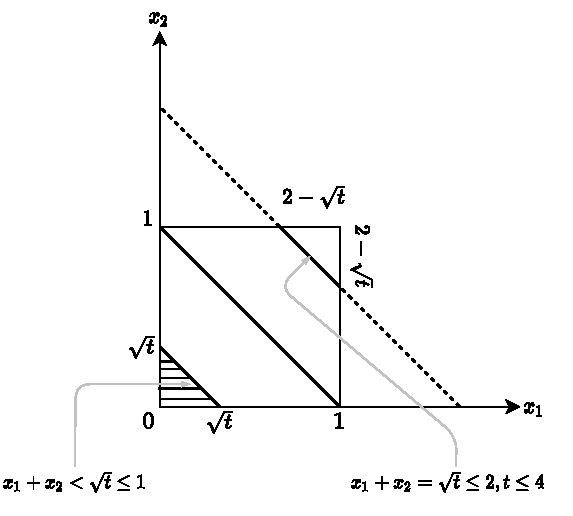
\includegraphics[scale=0.9]{./media/4_1.pdf}}
	\end{figure}
	
	Воспользуемся геометрическим определением интеграла для нахождения функции распределения данной случайной величины.
	
	При $t \in (0, 1]$ (площадь заштрихованной области):
	\[ F_{(\xi + \eta)^2} (t) = \int_{0}^{\sqrt{t}} dx_2 \int_{0}^{\sqrt{t} - x_2} dx_1 = \int_{0}^{\sqrt{t}} (\sqrt{t} - x_2) dx_2 = \frac{t}{2} \]
	
	При $t \in (1, 4]$ (вычитаем из площади квадрата $[0,1] \times [0,1]$ площадь треугольника со сторонами $2 - \sqrt{t}$):
	\[ F_{(\xi + \eta)^2} (t) = 1 - \int_{0}^{2 - \sqrt{t}} dx_2 \int_{0}^{2 - \sqrt{t} - x_2} dx_1 = \int_{0}^{2 - \sqrt{t}}(-\sqrt{t} - x_2 + 2) dx_2 = 1 - \frac{(\sqrt{r} - 2)^2}{2} \]
	Таким образом, функция распределения имеет следующий вид:
	\[
	F_{(\xi + \eta)^2} (t) =
	\begin{cases}
		0, &t \le 0 \\
		\frac{t}{2}, &t \in (0,1] \\
		1 - \frac{(\sqrt{t} - 2)^2}{2}, &t \in (1, 4] \\
		1, & t > 4
	\end{cases}
	\]
	График функции представлен ниже:
	\begin{figure}[H]
		\center{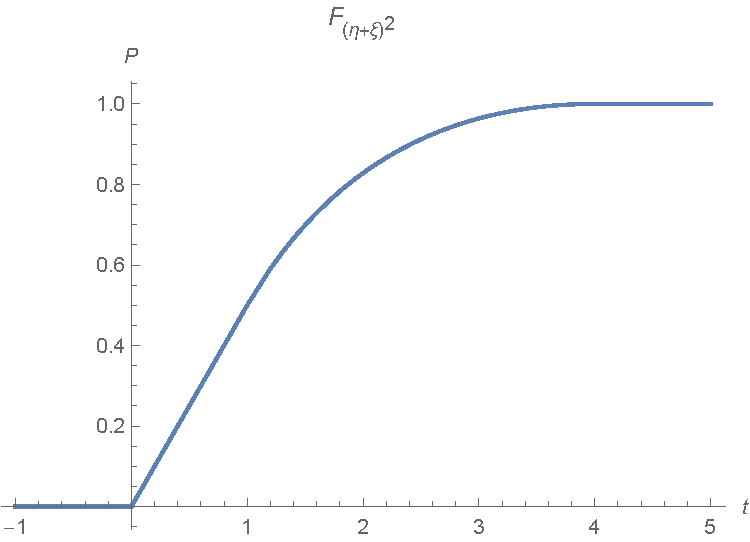
\includegraphics[scale=0.9]{./media/4_2.pdf}}
	\end{figure}
	\item[б)]
	
	Носитель распределения:
	\[ \supp (\xi) = \supp (\eta) = [0,1], 2\xi + 3 \eta < t, 0 < t \le 5 \]
	Функция распределения:
	\[ F_{2 \xi + 3 \eta} (t) = P(2 \xi + 3 \eta < t) \]
	Для удобства вычислений разобьём квадрат на несколько зон, а также введём несколько обозначений: $T_i$ - треугольник, используемый для вычислений в $i$-ой зоне; номера зон на рисунке помещены в синие рамки. \textcolor{Grey}{Границы интегрирования выражаются из носителя.}
	\begin{itemize}
		\item При $t \in (0, 2]$ функция распределения равна площади $T_1$, находящегося под прямой $2x_1+3x_2=t$:
		\[ F_{2\xi + 3\eta} (t) = \int_{0}^{\frac{t}{2}} dx_1 \int_{0}^{\frac{t-2x_1}{3}}dx_2 = \frac{t^2}{12} \]
		\item При $t \in (2, 3]$ функция распределения равна площади $T_1 - T_2$, где $T_2$ - площадь прямоугольника под вышеобозначенной прямой, но вне квадрата (зона 2).
		\[ F_{2\xi + 3\eta} (t) = \frac{t^2}{12} - \int_{0}^{\frac{t-2}{2}}dx_1 \int_{0}^{\frac{t-2x_1-2}{3}} dx_2 = \frac{t^2}{12} - \frac{1}{12} (t - 2)^2 = \frac{t-1}{3} \]
		\item При $t \in (3, 4]$ функция распределения равна разности площади квадрата и площади $T_3$, находящегося над прямой $2x_1 + 3x_2 = 4$ и образующего 4-ю область (находим 3-ю).
		\[ F_{2\xi + 3\eta} (t) = 1 - \int_{0}^{\frac{5-t}{2}}dx_1 \int_{0}^{\frac{5-2x_1-t}{3}} dx_2 = 1 - \frac{1}{12} (t - 5)^2 \]
	\end{itemize}
	\begin{figure}[H]
		\center{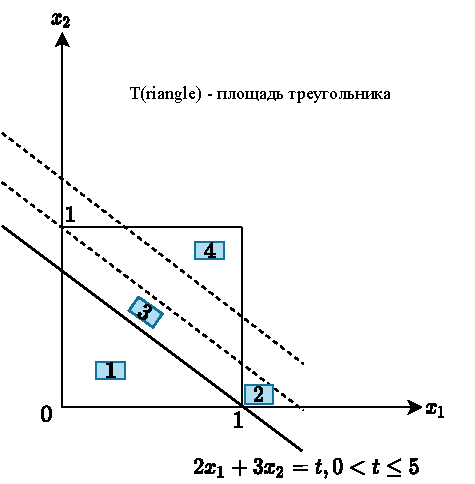
\includegraphics[scale=0.9]{./media/4_3.pdf}}
	\end{figure}
	Таком образом, функция распределения имеет следующий вид:
	\[
	F_{2\xi + 3\eta} (t) =
	\begin{cases}
		0, &t \le 0 \\
		\frac{t^2}{12}, &t \in (0, 2] \\
		\frac{t-1}{3}, &t \in (2, 3] \\
		1 - \frac{1}{12}(t-5)^2, &t \in (3, 5] \\
		1, &t > 5
	\end{cases}
	\]
	График функции представлен ниже:
	\begin{figure}[H]
		\center{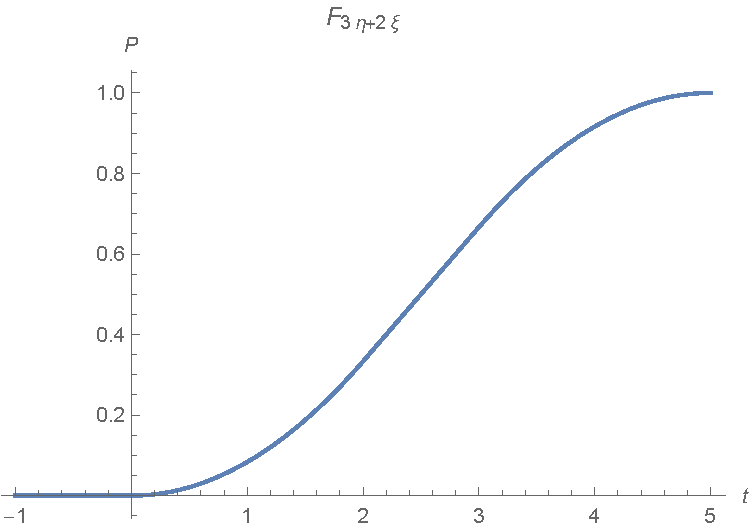
\includegraphics[scale=0.9]{./media/4_4.pdf}}
	\end{figure}

	\item[в)]
	Носитель распределения:
	\[ \supp (\xi) = \supp (\eta) = [0, 1], \xi^2 + \eta^2 < t, 0 < t < 2 \]
	Функция распределения:
	\[ F_{\xi^2 + \eta^2} = P(\xi^2 + \eta^2 < t) \]
	Заметим, что уравнение вида $x^2 + y^2 < z$ задаёт некоторую область внутри окружности радиуса $\sqrt{z}$ с центром в точке начала координат.
	
	Введём новое обозначение - $S_i$ - сектор, используемый в $i$-ой зоне.
	
	\begin{enumerate}
		\item[1.] При $t \in (0, 1]$ функция распределения равна площади сектора $S_1$, ограниченного прямыми координат и частью окружности с центром в $(0;0)$ и радиусом $t$. Требуемую площадь сектора найдём через следующую формулу:
		\[ S = \frac{\pi r^2 \alpha}{2 \pi} \]
		\[ F_{\xi^2 + \eta^2} (t) = \frac{t^2 \pi}{4} \]
		 \item[2.] При $t \in (1, 2]$ функция распределения равна сумме прямоугольника со сторонами 1 и $\sqrt{t-1}$, а также криволинейной трапеции, образованной под прямой $x_1^2 + x_2^2 = t, x_1 = \sqrt{t-1} \dots t$ с основанием $1 - \sqrt{t-1}$.
		 
		 Очевидно, что площадь прямоугольника равна $\sqrt{t-1}$. Площадь же криволинейной трапеции (выражаем $x_2$):
		 \[ \int_{\sqrt{t-1}}^{1} \sqrt{t-x_1^2} dx_1 = \frac{1}{2} \left( \sqrt{t-x^2} \cdot x + t \cdot \arcsin \frac{x}{\sqrt{t}} \right) \bigg|_{\sqrt{t-1}}^{1} = \]
		 \[ = \dots = \frac{1}{2} t \left( \arcsin \frac{1}{\sqrt{t}} - \arcsin \frac{\sqrt{t-1}}{\sqrt{t}} \right) \]
	\end{enumerate}
	\begin{figure}[H]
		\center{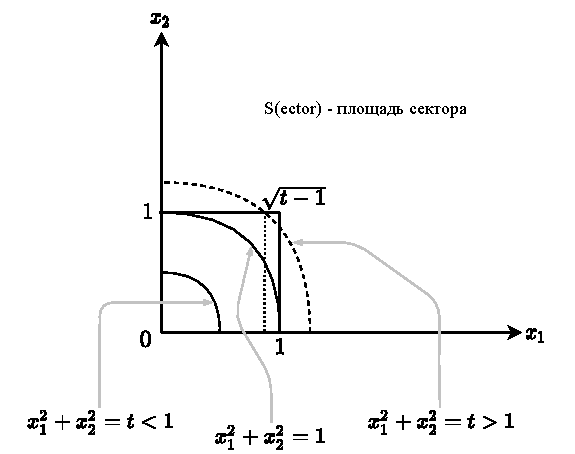
\includegraphics[scale=1.1]{./media/4_5.pdf}}
	\end{figure}
	Таким образом, функция распределения имеет следующий вид:
	\[
	F_{\xi^2 + \eta^2} (t) =
		\begin{cases}
		0, &t < 0 \\
		\frac{\pi t^2}{4}, &t \in (0, 1] \\
		\sqrt{t-1} + \frac{1}{2} t \left( \arcsin \frac{1}{\sqrt{t}} - \arcsin \frac{\sqrt{t-1}}{\sqrt{t}} \right), &t \in (1, 2] \\
		1, &t > 2
	\end{cases}
	\]
	График функции представлен ниже:
	\begin{figure}[H]
		\center{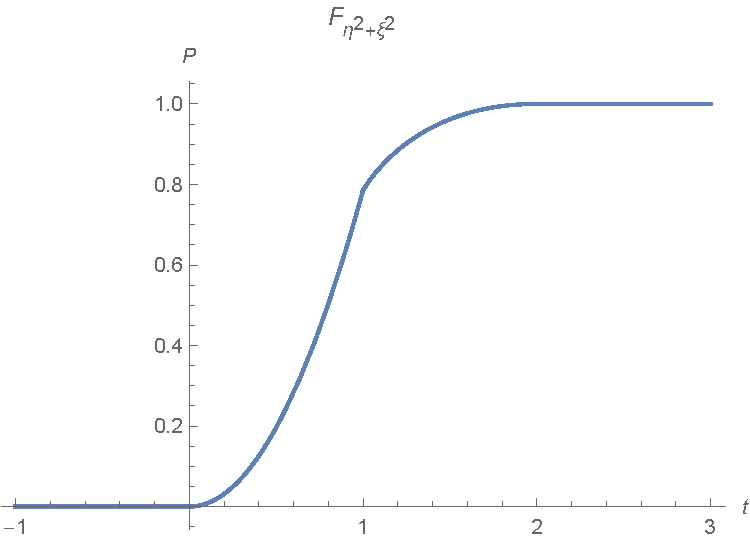
\includegraphics[scale=0.9]{./media/4_6.pdf}}
	\end{figure}

	Альтернативно,
	\[
	F_{\xi^2 + \eta^2} (t) =
	\begin{cases}
		0, &t < 0 \\
		\frac{\pi t^2}{4}, &t \in (0, 1] \\
		\sqrt{t-1} + \frac{t}{2} t \left( \arctan \frac{1}{\sqrt{t-1}} - \arctan (\sqrt{t-1}) \right), &t \in (1, 2] \\
		1, &t > 2
	\end{cases}
	\]
	Дифференцируем, преобразуем, находим плотность распределения
	\[
	p_{\xi^2 + \eta^2} =
	\begin{cases}
		\frac{\pi t}{2}, &t \in [0,1] \\
		\frac{1}{2} + \frac{\pi}{4} + \frac{1}{4 \sqrt{t-1}} - \arctan (\sqrt{t-1}), &t \in (1,2] \\
		1, &t > 2
	\end{cases}
	\]
	
	\textcolor{red}{(т.е. в окрестностях точек $t = 1$ и $t = 2$ функция распределения ведет себя не так как изображено
	на графике)}
	
	\item[г)]
	
	\[
	p_{\xi, \eta} (x, y) =
	\begin{cases}
		1, x, y \in [0, 1] \\
		0 - \text{ в остальных случаях}
	\end{cases}
	\]
	\[
	F_{\xi, \xi + \eta} (x_1, y_1) = P(\xi < x_1, \xi + \eta < y_1)
	\]
	\[
	\supp (x_1) = [0,1], ~~~ \supp (x_2) = [0,2]
	\]
	\begin{figure}[H]
		\center{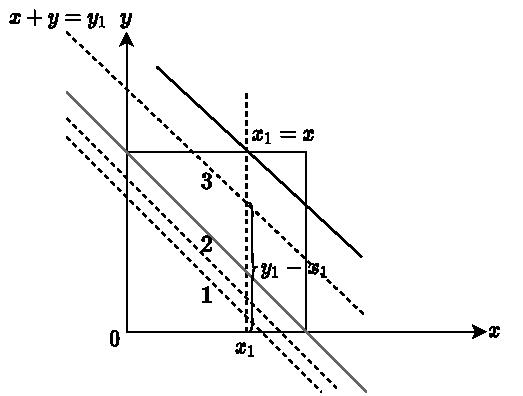
\includegraphics[scale=0.9]{./media/4_9.pdf}}
	\end{figure}
	
	На графике условие $x < x_1$ оставляет от квадрата прямоугольник от 0 до $x_1$ по оси $x$.
	
	Условие $x + y < y_1$ делает сечение прямоугольника, а итоговая фигура может быть либо треугольником (1 на рис.), либо трапецией (2 на рис.), либо прямоугольником с отсечённым треугольником (3 на рис.)
	
	Вычисляем функцию распределения $F_{\xi, \xi + \eta} (x, y)$ по областям (в скобках - форма области, площадь которой равна значению функции распределения).
	\begin{enumerate}
		\item $\{ x \le 0 \} \cup \{ y \le 0 \}$ (пустое множество): $F_{\xi, \xi + \eta} (x, y) = 0$;
		\item $\{ x \in (0, 1] \} \cap \{ 0 < y \le x \}$ (треугольник): $F_{\xi, \xi + \eta} (x, y) = P(\xi + \eta < y) = \frac{y^2}{2}$;
		\item $\{ x \in (0, 1] \} \cap \{ x < y \le x + 1 \}$ (трапеция): $F_{\xi, \xi + \eta} (x, y) = \left(y-\frac{x}{2}\right)x$;
		\item $\{ x \in (0, 1] \} \cap \{ y > x + 1 \}$ (прямоугольник): $F_{\xi, \xi + \eta} (x, y) = P(\xi < x) = x$;
		\item $\{ x > 1 \} \cap \{ y \in (0, 1] \}$ (треугольник): $F_{\xi, \xi + \eta} (x, y) = P(\xi + \eta < y) = \frac{y^2}{2}$;
		\item $\{ x > 1 \} \cap \{ y \in (1, 2] \}$ (прямоугольник с отсечённым треугольником): $F_{\xi, \xi + \eta} (x, y) = P(\xi + \eta < y) = 1 - \frac{(2-y)^2}{2}$;
		\item $\{ x > 1 \} \cap \{ y > 2 \}$ (квадрат $[0, 1]^2$): $F_{\xi, \xi + \eta} (x, y) = 1$.
	\end{enumerate}
	Таким образом,
	\[
	F_{\xi, \xi + \eta} (x, y) =
	\begin{cases}
		0, &x \le 0 \lor y \le 0 \\
		\frac{y^2}{2}, &x \in (0, 1], 0 < y \le x \lor x > 1, y \in (0, 1] \\
		\left( y - \frac{x}{2} \right) x, &x \in (0, 1], x < y \le x + 1 \\
		x, &x \in (0, 1], y > x + 1 \\
		1 - \frac{(2-y)^2}{2}, &x > 1, y \in (1, 2] \\
		1, &x > 1, y > 2
	\end{cases}
	\]
	Берем смешанную производную, получаем плотность распределения
	\[
	p_{\xi, \xi + \eta} (x, y) =
	\begin{cases}
		1, x \in [0, 1], x \le y \le x + 1 \\
		0 - \text{ в остальных случаях}
	\end{cases}
	\]
	
\end{enumerate}

\section*{Задача 5 (СГТВ раздел 3 - задача 6).}

\noindent\textit{\textbf{Условие:}}

Совместная плотность распределения случайных величин $\xi$ и $\eta$ имеет вид:
\[
p_{\xi, \eta} (x, y) =
\begin{cases}
	c x(x+y), 0 \le x \le y \le 1 \\
	0 - \text{ в остальных случаях}
\end{cases}
\]
Найти константу $c$. Вычислить распределение величины $\exp (3 \xi + 2 \eta)$.

\noindent\textit{\textbf{Решение:}}

\begin{itemize}
	\item  Для того, чтобы найти плотность распределения одной из компонент вектора, надо проинтегрировать плотность по всем остальным переменным, т.е. при каждом $x \in \mathbb{R}$.
	\[ \int_{- \infty}^{\infty} \int_{- \infty}^{\infty} p_{\xi, \eta} (x, y) dxdy = 1 \]
	\[ \int_{0}^{1} dy \int_{0}^{y} c x(x+y) dx = \dots \]
	Решаем внутренний интеграл:
	\[ \int_{0}^{y} c x(x+y) dx = c \int_{0}^{y} x(x+y) dx =
	\left| \begin{smallmatrix} u = x+y & du = dx \\ u = y + 0 & u = y+y=2y \end{smallmatrix} \right|
	= c \int_{y}^{2y} u^2 du - c y \int_{y}^{2y} udu = \frac{5cy^3}{6}
	\]
	\[ \dots = \int_{0}^{1} \frac{5cy^3}{6} dy = \frac{5c}{6} \int_{0}^{1} y^3 dy = \frac{5c}{24} = 1 \Rightarrow c = \frac{24}{5} \]
	\item Функция распределения в данном случай имеет следующий вид:
	\[ F_{3 \xi + 2 \eta} = P(3\xi + 2 \eta < t) \]
	Представь данный случай графически.
	\begin{figure}[H]
		\center{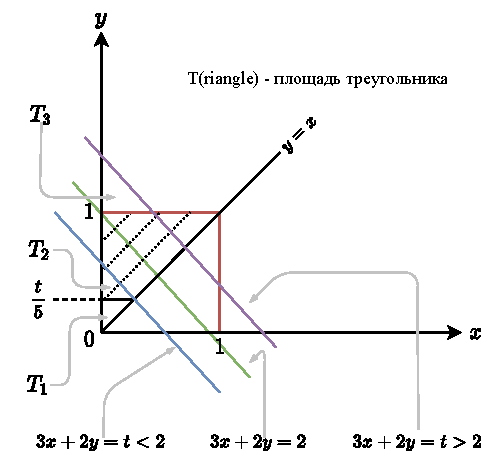
\includegraphics[scale=0.9]{./media/4_7.pdf}}
	\end{figure}
	На данном изображении используется уже введённое условное обозначение площади треугольника $i$-ой зоны, а также дополнительное построение в виде прямой, заданной уравнением $y=x$. Также на рисунке обозначена точка пересечения прямых с координатам $\left(\frac{t}{5}; \frac{t}{5}\right)$, заданных уравнениями обозначенной прямой и функции распределения.
	\begin{itemize}
		\item При $t \in (0, 2]$ (до зелёной лини, включая синюю) функция распределения будет равняться сумме $T_1 + T_2:$
		\[ F_{3 \xi + 2 \eta} (t) = \int_{0}^{\frac{t}{5}}dy \int_{0}^{y} \frac{24x(x+y)}{5} dx + \int_{\frac{t}{5}}^{\frac{t}{2}} dy \int_{0}^{\frac{t-2y}{3}} \frac{24x(x+y)}{5} dx = \dots \]
		\[ \underset{wolfram}{\dots =} \frac{t^4}{625} + \frac{9t^2}{2500} = \frac{13t^4}{2500} \]
		\item При $t \in (2, 5]$ интересующая нас область будет определяться как разность $T$, образованного прямыми, заданных уравнениями $y=x, x=0$, прямой функции распределения (заштрихованная область на рисунке) и $T_3$.
		Верхнюю границу интегрирования внутреннего интеграла получаем путём выражения $3x+2y=t \Rightarrow x = \frac{t - 2y}{3}$.
		\[  F_{3 \xi + 2 \eta} (t) = \frac{13t^4}{2500} - \int_{1}^{\frac{t}{2}}dy \int_{0}^{\frac{t-2y}{3}} \frac{24x(x+y)}{5} dx = \underset{wolfram}{\dots = } -\frac{131 t^4}{16875}+\frac{8 t^3}{135}-\frac{2 t^2}{45}-\frac{16 t}{135}+\frac{4}{27} \]
	\end{itemize}
	Таким образом, функция распределения имеет следующий вид:
	\[
	F_{3 \xi + 2 \eta} =
	\begin{cases}
		0, &t \le 0 \\
		\frac{13t^4}{2500}, & t \in (0,2] \\
		-\frac{131 t^4}{16875}+\frac{8 t^3}{135}-\frac{2 t^2}{45}-\frac{16 t}{135}+\frac{4}{27}, &t \in (2, 5] \\
		1, &t > 5
	\end{cases}
	\]
	\[ \Downarrow \]
	\[
	F_{\exp(3 \xi + 2 \eta)} = F_{3\xi+2\eta}(\ln t) =
	\begin{cases}
		0, &t \le 1 \\
		\frac{13 \ln t^4}{2500}, &t \in (1, e^2] \\
		-\frac{131 \ln (t)^4}{16875}+\frac{8 \ln (t)^3}{135}-\frac{2 \ln (t)^2}{45}-\frac{16 \ln (t)}{135}+\frac{4}{27}, &t \in (e^2, e^5] \\
		1, & t > e^5
	\end{cases}
	\]
\end{itemize}

\section*{Задача 6 (СГТВ раздел 3 - задача 7).}

\noindent\textit{\textbf{Условие:}}

Плотность распределения случайного вектора $(\xi, \eta)$ имеет вид:
\[
p_{\xi, \eta} (x, y) =
\begin{cases}
	c \exp (-(x+y)), 0 \le y \le x \\
	0 - \text{ в остальных случаях}
\end{cases}
\]
Найти константу $c$. Вычислить распределение разности $\xi - \eta$.

\noindent\textit{\textbf{Решение:}}

\begin{itemize}
	\item Для того, чтобы найти плотность распределения одной из компонент вектора, надо проинтегрировать плотность по всем остальным переменным, т.е. при каждом $x \in \mathbb{R}$.
	\[ \int_{- \infty}^{\infty} \int_{- \infty}^{\infty} p_{\xi, \eta} (x, y) dxdy = 1 \]
	\[ \int_{0}^{\infty}dx \int_{0}^{x} c \cdot \exp (-(x+y)) dy = \dots \]
	Решаем внутренний интеграл:
	\[ \int_{0}^{x} c \cdot \exp (-(x+y)) dy = c \int_{0}^{x} c \cdot e^(-x-y) = 
	\left| \begin{smallmatrix} u = -x-y; & du = -dy \\ u = -x-0; & u = -x-x=-2x \end{smallmatrix} \right| = 
	(-ce^u) \bigg|_{u=-x}^{-2x} = \]
	\[ = (-ce^{-2x})-(ce^{-x})=ce^{-2x}(e^x-1) = ce^{-2x}(e^x-1) \]
	\[ \dots = \int_{0}^{\infty} ce^{-2x}(e^x-1) dx = c \int_{0}^{\infty} e^{-2x}(e^x-1) dx = 
	\left| \begin{smallmatrix} u = e^x & du = e^xdx \\ u = e^0 = 1 & u = \infty \end{smallmatrix} \right| =
	c \int_{1}^{\infty} \frac{u-1}{u^3} du =\]
	\[ = \left| \begin{smallmatrix} s = u-1 & ds = du \\ s = 1-1=0 & s = \infty \end{smallmatrix} \right| =
	c \int_{0}^{\infty} \frac{s}{s^3 + 3s^2 + 3s + 1}ds = c \int_{0}^{\infty} \frac{s}{(s+1)^3} = 
	 \]
	 \[ c \int_{0}^{\infty} \frac{1}{(s+1)^2} ds - c \int_{0}^{\infty} \frac{1}{(s+1)^3} ds = \dots = c - \frac{c}{2} = \frac{c}{2} = 1 \Rightarrow c = 2 \]
	 \item Функция распределения имеет следующий вид:
	 \[ F_{\xi} = P(\xi - \eta < t) \]
	 В текущем случае область интегрирования будет задаваться тремя прямыми с уравнениями: $x=0, y=x, x-y=t$. Данный факт отражён на рисунке ниже (заштрихованная область).
	 \begin{figure}[H]
	 	\center{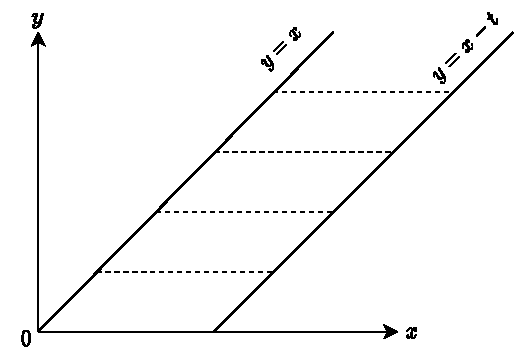
\includegraphics[scale=0.9]{./media/4_8.pdf}}
	 \end{figure}
 	При $t \in (0, +\infty)$ функция распределения имеет следующий вид:
 	\[ F_{\xi - \eta}(t) = \int_{0}^{\infty} dx \int_{0}^{x} c \exp (-(x+y)) dy - \int_{t}^{\infty} dx \int_{0}^{x-t} c \exp (-(x+y)) dy = \]
 	\[ = \int_{0}^{\infty} dx \infty_{0}^{x} 2 e^{-x-y} dy - \int_{t}^{\infty} dx \int_{0}^{x-t} 2e^{-x-y}dy = \]
 	\[ = \int_{0}^{\infty} (2e^{-x} - 2e^{-2x}) dx - \int_{0}^{\infty} (2e^{-x}-2e^{t-2x})dx = \]
 	\[ = 2 - 2 \int_{0}^{\infty} e^{-2x} dx - 2e^{-t} - 2 \int_{t}^{\infty} e^{t-2x} dx = \]
 	\[ = 2 - 1 - e^{-t} = 1 - e^{-t} \]
 	Таким образом, функция имеет следующий вид:
 	\[
 	F_{\xi - \eta} (t) =
 	\begin{cases}
 		0, &t \le 0 \\
 		1 - e^{-t}, &t > 0
 	\end{cases}
 	\]
\end{itemize}

\end{document} 